%%%%%%%%%%%%%%%%%%%%%%%%%%%%%%%%%%%%%%%%%%%%%%
%                insertmeeting
% 1) Title (something creative & funny?)
% 2) Date (MM/DD/YYYY)
% 3) Location (ex. Hagerty High School)
% 4) People/Committees Present 
% 5) Picture 
% 6) Start Time & Stop Time (ex. 12:30AM to 4:30PM)
%%%%%%%%%%%%%%%%%%%%%%%%%%%%%%%%%%%%%%%%%%%%%%
\insertmeeting 
	{Sponsor Sitdown} 
	{10/21/21}
	{Hagerty High School}
	{Annika, Clayton, Falon, Jensen, Nathan, Ritam, Samantha}
	{Images/RobotPics/robot.jpg}
	{2:30 - 4:30}
	
\hhscommittee{Outreach}
\noindent\hfil\rule{\textwidth}{.4pt}\hfil
\subsubsection*{Goals}
\begin{itemize}
    \item The goal for the Outreach Committee was to make significant progress on letters for many of our sponsors from current and previous years. This includes writing and editing thank you letters and letters asking for sponsorships. 

\end{itemize} 

\noindent\hfil\rule{\textwidth}{.4pt}\hfil

\subsubsection*{Accomplishments}
During today's meeting, we specified the "Thank You" letter template to apply to the 11 different organizations and companies that had provided us with donations in the previous season. Many of these donations included monetary contributions, discounts on products, and free items like software, REV Hubs, batteries, and a TV. The sponsor thank you letters detail how the contributions have benefitted our team, while giving each donor a review of the past season and our achievements. We made sure to include that our team is continuing on in this season of Freight Frenzy, and that their continued support would be greatly appreciated. The team decided that once the letters are printed, that we should sign them by hand, as opposed to making digital signatures. We decided to do this, along with including a group picture of our team, to establish more sentiment with the companies and organizations that have provided us with generosity. By doing so, we hope that our connection with our sponsors will be reinforced, especially after the 2020-2021 season which had taken a toll on our ability to communicate with them.

\hhscommittee{Hardware}
\noindent\hfil\rule{\textwidth}{.4pt}\hfil
\subsubsection*{Goals}
\begin{itemize}
    \item Redesign the wheel holder to be flat for improved odometry

\end{itemize} 

\noindent\hfil\rule{\textwidth}{.4pt}\hfil

\subsubsection*{Accomplishments}
Recently, we’ve been thinking a lot about how to effectively add odometry to the robot, and after adding encoders to the front wheel, our software committee thought of a potential problem with the current steering measurement system. In order to make the robot turn more steadily, we initially placed the fork at a 10 degree angle to the horizontal, which was a good solution without odometry, but now we think it might interfere with our position calculation. As our software committee told us,with the wheel’s axis of rotation at an angle, turning the wheel 90 degrees might not have the same turning radius as if the axis or rotation was perpendicular to the ground. When we thought about it, this actually made a lot of sense. Increasing the angle makes turning more steady by increasing the amount you need to turn the wheel to make a turn of the same radius. This means that small adjustments are less detrimental to the vehicle's turn, making it seem more steady. Because this change will make the odometry much more difficult to test and tune, we decided to redesign the wheel holder to hold the wheel perpendicular to the ground. Although this could make our steering worse, we don’t think it will have enough of an effect to outweigh the benefits of odometry. Even in the worst case scenario, if we need to change the holder back to an angle, the dovetail slot we put onto the drivetrain will make it easy to switch out.
With that decision made, we began designing a front wheel. We started out by making a similar basic shape to the angled wheel holder, but made the holder parallel to the ground. Because we don't have the angle of adding height to the holder and keeping the wheel higher off the ground, we had to add a bend so that the rest of the drivetrain is still level with the ground (Figure \ref{fig:pic1}). From there we added some lightening holes and a rounded front to reduce weight while maintaining stability (Figure \ref{fig:pic2}). While designing, we noticed that the unused space at the back of the holder was large enough to fit a small servo, making this the perfect place to put the steering servo. We added some holes to the wheel holder and created a plate to attach a servo to. With all of the new parts designed, we added these parts and a Hi-Tec HS-225 servo into an assembly, confirming that all of the parts fit together properly (Figure \ref{fig:pic3}).

\begin{figure}[ht]
\centering
\begin{minipage}[b]{.48\textwidth}
  \centering
  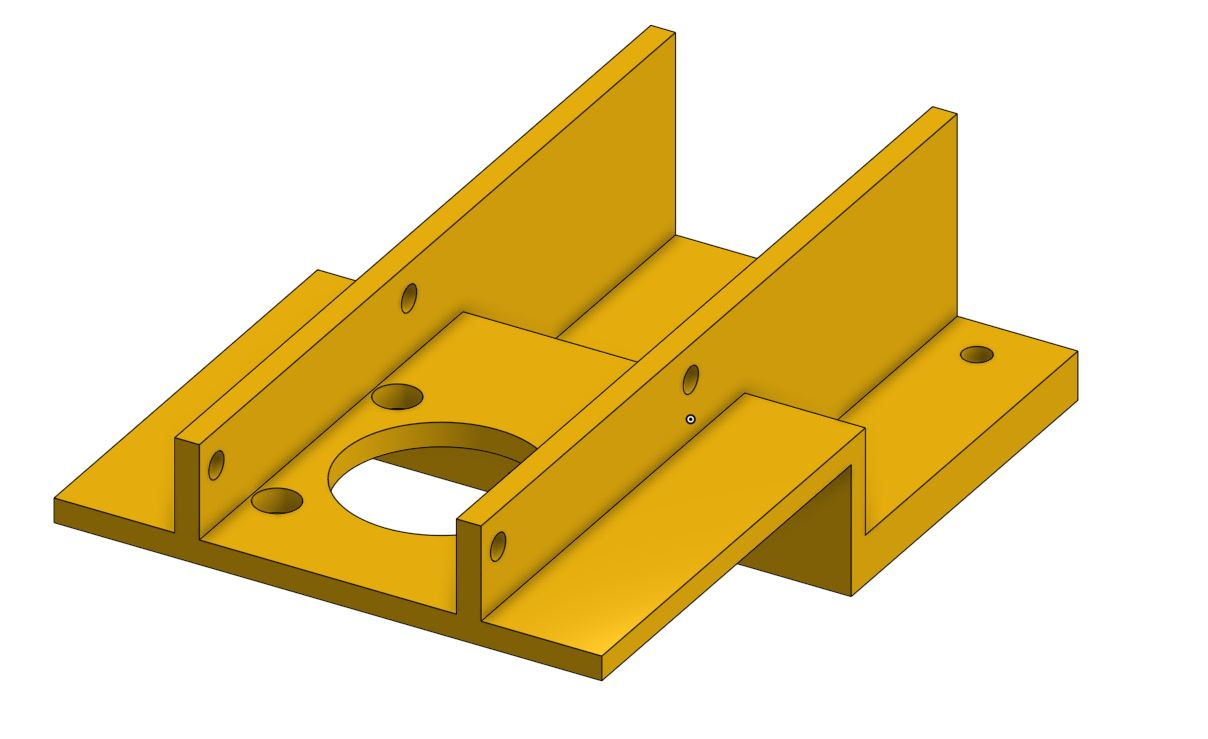
\includegraphics[width=0.95\textwidth]{Meetings/October/10-21-21/10-21-21_CAD_Figure1 - Nathan Forrer.JPG}
  \caption{Moving the wheel higher.}
  \label{fig:pic1}
\end{minipage}%
\hfill%
\begin{minipage}[b]{.48\textwidth}
  \centering
  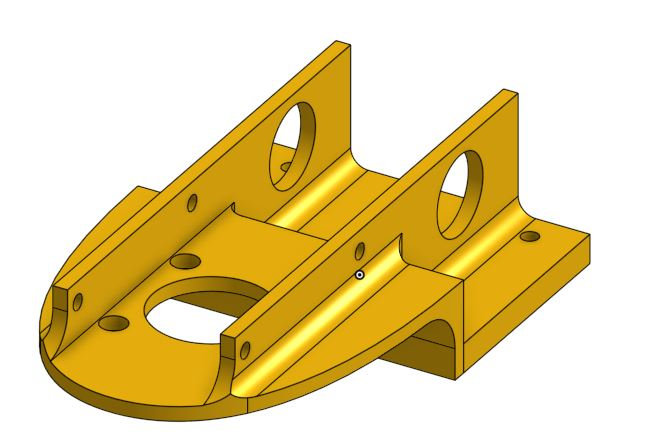
\includegraphics[width=0.95\textwidth]{Meetings/October/10-21-21/10-21-21_CAD_Figure2 - Nathan Forrer.JPG}
  \caption{Lightening holes and rounded front.}
  \label{fig:pic2}
\end{minipage}
\end{figure}

\begin{figure}[htp]
\centering
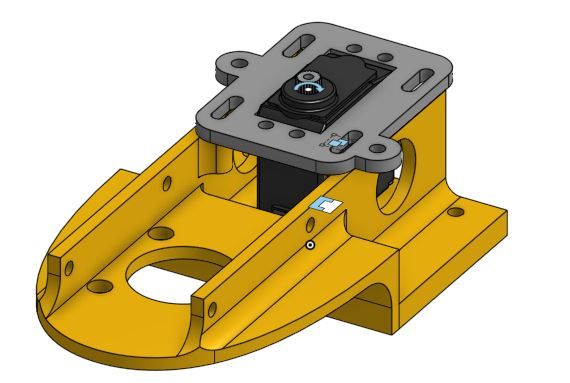
\includegraphics[width=0.95\textwidth, angle=0]{Meetings/October/10-21-21/10-21-21_CAD_Figure3 - Nathan Forrer.JPG}
\caption{The final assembly.}
\label{fig:pic3}
\end{figure}


\whatsnext{
\begin{itemize}
    \item During the next meeting, we plan on printing out the letters and signing them. Afterwards, we will be able to send them out to all of the companies who donated to us, making our work as a team possible.
    \item Design extending arm mechanism
	\item Recreate intake to fit on new arm
	\item Test drivetrain
\end{itemize} 
}

